\chapter{复分析}

复分析研究复变量函数的微分、积分、级数展开和奇点结构。它与实分析的一个重要差别在于：复可微性比实可微性强得多。一个函数只要在区域内复可微，就会自动具有幂级数展开，并且受到 Cauchy 积分公式、最大模原理、留数定理等强有力结果的约束。

本章的目标不是穷尽复分析的全部内容，而是建立一条从复数、复平面、复可微性到 Cauchy 理论和留数计算的基本路径。

\section{复数与复平面}

\subsection{代数定义}

\begin{definition}[复数]
复数是形如
\[
    z=a+bi
\]
的对象，其中 $a,b\in\mathbb{R}$，且 $i^2=-1$。$a$ 称为实部，$b$ 称为虚部，记作
\[
    \operatorname{Re}z=a,
    \qquad
    \operatorname{Im}z=b.
\]
复数集记作 $\mathbb{C}$。
\end{definition}

复数的加法和乘法按形式运算并使用 $i^2=-1$ 化简：
\[
    (a+bi)+(c+di)=(a+c)+(b+d)i,
\]
\[
    (a+bi)(c+di)=(ac-bd)+(ad+bc)i.
\]
由此可见，$\mathbb{C}$ 是一个域，并且包含 $\mathbb{R}$ 作为子域。

\begin{definition}[共轭与模]
设 $z=a+bi$。复共轭定义为
\[
    \overline{z}=a-bi,
\]
模定义为
\[
    |z|=\sqrt{a^2+b^2}.
\]
\end{definition}

\begin{proposition}[基本恒等式]
对任意 $z,w\in\mathbb{C}$，有
\[
    z\overline z=|z|^2,
    \qquad
    |zw|=|z||w|,
    \qquad
    \overline{z+w}=\overline z+\overline w,
\]
并且当 $z\ne0$ 时，
\[
    z^{-1}=\frac{\overline z}{|z|^2}.
\]
\end{proposition}

\subsection{几何解释}

复数 $z=a+bi$ 可以看作平面点 $(a,b)$。因此，$\mathbb{C}$ 与 $\mathbb{R}^2$ 在集合和几何直观上可以对应起来，这个平面称为\textbf{复平面}。在这个解释下，$|z|$ 就是点 $z$ 到原点的欧氏距离。

\begin{definition}[辐角]
若 $z\ne0$，则满足
\[
    z=|z|(\cos\theta+i\sin\theta)
\]
的角 $\theta$ 称为 $z$ 的一个\textbf{辐角}，记作 $\arg z$。由于角可以相差 $2\pi$ 的整数倍，辐角通常是多值的。
\end{definition}

\begin{definition}[极坐标形式]
若 $z\ne0$，则可以写作
\[
    z=r(\cos\theta+i\sin\theta),
    \qquad r=|z|>0.
\]
这称为 $z$ 的极坐标形式。
\end{definition}

\subsection{Euler 公式}

\begin{theorem}[Euler 公式]
对任意实数 $\theta$，有
\[
    e^{i\theta}=\cos\theta+i\sin\theta.
\]
\end{theorem}

这个公式把指数函数、三角函数与复数乘法统一起来，是复分析中最重要的公式之一。

\begin{corollary}[指数形式]
任意非零复数都可以写成
\[
    z=re^{i\theta},
    \qquad r=|z|>0.
\]
\end{corollary}

\newpage

\begin{proposition}[极坐标形式下的乘法]
若
\[
    z_1=r_1e^{i\theta_1},
    \qquad
    z_2=r_2e^{i\theta_2},
\]
则
\[
    z_1z_2=r_1r_2e^{i(\theta_1+\theta_2)}.
\]
因此，复数相乘对应于模相乘、辐角相加。
\end{proposition}

\begin{theorem}[De Moivre 公式]
对任意整数 $n$，有
\[
    (\cos\theta+i\sin\theta)^n
    =\cos(n\theta)+i\sin(n\theta).
\]
\end{theorem}

\begin{example}[单位根]
方程 $z^n=1$ 的全部解为
\[
    z_k=e^{2\pi i k/n},
    \qquad k=0,1,\dots,n-1.
\]
这些点均匀分布在单位圆上，构成正 $n$ 边形的顶点。
\end{example}

\section{复平面的拓扑}

因为 $\mathbb{C}$ 可与 $\mathbb{R}^2$ 识别，复平面继承了通常的欧氏拓扑。对 $z_0\in\mathbb{C}$ 和 $r>0$，定义开圆盘
\[
    D(z_0,r)=\{z\in\mathbb{C}:|z-z_0|<r\}.
\]

\begin{definition}[开圆盘]
集合 $D(z_0,r)$ 称为以 $z_0$ 为中心、半径为 $r$ 的开圆盘。
\end{definition}

\begin{definition}[区域]
复平面中的非空开连通集称为\textbf{区域}。
\end{definition}

\begin{definition}[极限与连续性]
设 $f$ 定义在 $z_0$ 的某个去心邻域中。若存在 $L\in\mathbb{C}$，使得对任意 $\varepsilon>0$，存在 $\delta>0$，当
\[
    0<|z-z_0|<\delta
\]
时有
\[
    |f(z)-L|<\varepsilon,
\]
则称
\[
    \lim_{z\to z_0}f(z)=L.
\]
若 $f$ 在 $z_0$ 有定义且
\[
    \lim_{z\to z_0}f(z)=f(z_0),
\]
则称 $f$ 在 $z_0$ 连续。
\end{definition}

这里的极限要求 $z$ 从复平面中任意方向趋向 $z_0$。因此，复变量极限比一元实函数极限更严格。

\section{复可微性}

\subsection{复导数的定义}

\begin{definition}[复导数]
设 $f$ 在 $z_0$ 的某个邻域中有定义。如果极限
\[
    f'(z_0)=\lim_{h\to0}\frac{f(z_0+h)-f(z_0)}{h}
\]
存在，则称 $f$ 在 $z_0$ 处复可微，并称该极限为 $f$ 在 $z_0$ 的复导数。
\end{definition}

由于 $h\in\mathbb{C}$ 可以沿任意方向趋于 $0$，复可微性实际上包含了许多方向导数的一致性要求。

\begin{example}
函数 $f(z)=z^2$ 在整个复平面上可微，且
\[
    f'(z)=2z.
\]
这可以直接由差商计算得到：
\[
    \frac{(z+h)^2-z^2}{h}=2z+h\to2z.
\]
\end{example}

\begin{example}[复共轭函数]
函数 $f(z)=\overline z$ 在任何点都不复可微。因为在 $z_0$ 处，差商为
\[
    \frac{\overline{z_0+h}-\overline{z_0}}{h}=\frac{\overline h}{h}.
\]
若 $h$ 沿实轴趋于 $0$，该比值趋于 $1$；若 $h$ 沿虚轴趋于 $0$，该比值趋于 $-1$。极限不存在。
\end{example}

\subsection{全纯函数}

\begin{definition}[全纯函数]
设 $\Omega\subseteq\mathbb{C}$ 是开集。如果函数 $f:\Omega\to\mathbb{C}$ 在 $\Omega$ 中每一点都复可微，则称 $f$ 在 $\Omega$ 上\textbf{全纯}。
\end{definition}

\begin{proposition}[求导法则]
全纯函数满足通常的求导法则：若 $f,g$ 在 $\Omega$ 上全纯，则 $f+g$、$fg$ 全纯；若 $g$ 没有零点，则 $f/g$ 全纯；复合函数也满足链式法则
\[
    (g\circ f)'(z)=g'(f(z))f'(z).
\]
\end{proposition}

\section{Cauchy--Riemann 方程}

设
\[
    f(z)=u(x,y)+iv(x,y),
    \qquad z=x+iy,
\]
其中 $u,v$ 是实值函数。复可微性要求沿实方向和虚方向得到的差商极限一致。

沿实方向，
\[
    f'(z)=u_x+iv_x.
\]
沿虚方向，
\[
    f'(z)=\frac{u_y+iv_y}{i}=v_y-iu_y.
\]
比较实部和虚部得到 Cauchy--Riemann 方程。

\begin{theorem}[Cauchy--Riemann 方程]
若 $f=u+iv$ 在点 $z=x+iy$ 处复可微，并且 $u,v$ 的偏导数存在，则
\[
    u_x=v_y,
    \qquad
    u_y=-v_x.
\]
\end{theorem}

\begin{theorem}[充分条件]
若 $u,v$ 在开集 $\Omega$ 上具有连续偏导数，并且满足 Cauchy--Riemann 方程，则 $f=u+iv$ 在 $\Omega$ 上全纯。
\end{theorem}

\begin{example}
函数 $f(z)=z^2$ 可写作
\[
    f(x+iy)=x^2-y^2+2xyi.
\]
此时
\[
    u=x^2-y^2,
    \qquad
    v=2xy.
\]
于是
\[
    u_x=2x=v_y,
    \qquad
    u_y=-2y=-v_x,
\]
满足 Cauchy--Riemann 方程。
\end{example}

\begin{example}
函数 $f(z)=\overline z=x-iy$ 对应 $u=x,v=-y$。此时
\[
    u_x=1,
    \qquad
    v_y=-1,
\]
不满足 Cauchy--Riemann 方程，因此不全纯。
\end{example}

\subsection{几何意义}

\begin{definition}[保角映射]
若全纯函数 $f$ 在点 $z_0$ 满足 $f'(z_0)\ne0$，则它在 $z_0$ 附近保持曲线夹角及其方向，称为在该点\textbf{保角}。
\end{definition}

直观上，非零复导数的作用是“旋转加伸缩”。这也是复函数比一般二维实函数更刚性的原因之一。

\section{初等全纯函数}

\subsection{指数函数与三角函数}

\begin{definition}[复指数函数]
复指数函数定义为
\[
    e^z=e^x(\cos y+i\sin y),
    \qquad z=x+iy.
\]
\end{definition}

\begin{proposition}
复指数函数在整个复平面上全纯，且
\[
    (e^z)'=e^z.
\]
并且有周期性
\[
    e^{z+2\pi i}=e^z.
\]
\end{proposition}

\begin{definition}[复正弦与复余弦]
定义
\[
    \sin z=\frac{e^{iz}-e^{-iz}}{2i},
    \qquad
    \cos z=\frac{e^{iz}+e^{-iz}}{2}.
\]
\end{definition}

\begin{proposition}
函数 $\sin z$ 和 $\cos z$ 都是整函数，并满足
\[
    (\sin z)'=\cos z,
    \qquad
    (\cos z)'=-\sin z.
\]
同时仍有恒等式
\[
    \sin^2 z+\cos^2 z=1.
\]
\end{proposition}

\subsection{复对数}

复对数比实对数复杂，因为复指数函数具有周期 $2\pi i$。若 $z=re^{i\theta}$，则对数的自然候选为
\[
    \log z=\ln r+i\theta.
\]
但 $\theta$ 可以加上 $2\pi k$，所以复对数通常是多值的。

\begin{definition}[多值对数]
对 $z\ne0$，复对数定义为多值函数
\[
    \log z=\ln|z|+i(\arg z+2\pi k),
    \qquad k\in\mathbb{Z}.
\]
\end{definition}

\begin{definition}[主值分支]
令 $\operatorname{Arg}z\in(-\pi,\pi]$ 表示主辐角。复对数主值定义为
\[
    \operatorname{Log}z=\ln|z|+i\operatorname{Arg}z.
\]
\end{definition}

\begin{remark}
复对数不能在整个 $\mathbb{C}\setminus\{0\}$ 上选取单值连续分支。这一现象反映了穿孔平面的拓扑结构。
\end{remark}

\section{复积分}

\subsection{曲线与围道积分}

\begin{definition}[路径]
一条路径是连续映射
\[
    \gamma:[a,b]\to\mathbb{C}.
\]
如果 $\gamma$ 分段连续可微，则称它为分段光滑路径。
\end{definition}

\begin{definition}[围道积分]
设 $f$ 在路径 $\gamma$ 的像上连续，且 $\gamma$ 分段光滑。定义
\[
    \int_\gamma f(z)\,dz
    =\int_a^b f(\gamma(t))\gamma'(t)\,dt.
\]
\end{definition}

\begin{example}
若 $\gamma(t)=e^{it}$，$0\le t\le2\pi$，则
\[
    \int_\gamma \frac1z\,dz
    =\int_0^{2\pi}\frac1{e^{it}}ie^{it}\,dt
    =2\pi i.
\]
这个计算是复分析中许多结果的原型。
\end{example}

\begin{proposition}[估计引理]
若 $|f(z)|\le M$ 对 $z\in\gamma$ 成立，且 $\gamma$ 的长度为 $L$，则
\[
    \left|\int_\gamma f(z)\,dz\right|\le ML.
\]
\end{proposition}

\subsection{原函数}

\begin{definition}[原函数]
若在区域 $\Omega$ 上存在全纯函数 $F$，使得
\[
    F'(z)=f(z),
\]
则称 $F$ 是 $f$ 的原函数。
\end{definition}

\begin{theorem}[复线积分基本定理]
若 $F'=f$，则对任意从 $z_0$ 到 $z_1$ 的分段光滑路径 $\gamma$，有
\[
    \int_\gamma f(z)\,dz=F(z_1)-F(z_0).
\]
特别地，若 $\gamma$ 是闭路径，则
\[
    \int_\gamma f(z)\,dz=0.
\]
\end{theorem}

\section{Cauchy 定理与 Cauchy 积分公式}

\begin{theorem}[Cauchy 定理，简单形式]
设 $\Omega$ 是单连通区域，$f$ 在 $\Omega$ 上全纯。若 $\gamma$ 是 $\Omega$ 中的闭合分段光滑路径，则
\[
    \int_\gamma f(z)\,dz=0.
\]
\end{theorem}

\begin{remark}
Cauchy 定理说明，全纯函数沿闭曲线的积分常常为零。它是复分析中由局部可微性推出整体积分性质的核心桥梁。
\end{remark}

\begin{theorem}[Cauchy 积分公式]
设 $f$ 在包含闭圆盘 $\overline{D(a,r)}$ 的开集上全纯。若 $|z-a|<r$，则
\[
    f(z)=\frac1{2\pi i}\int_{|\zeta-a|=r}\frac{f(\zeta)}{\zeta-z}\,d\zeta.
\]
\end{theorem}

这个公式极其重要：区域内部任一点的函数值，可以由边界上的积分完全决定。

\begin{theorem}[导数形式的 Cauchy 积分公式]
在同样条件下，对任意 $n\ge0$，有
\[
    f^{(n)}(z)=\frac{n!}{2\pi i}\int_{|\zeta-a|=r}\frac{f(\zeta)}{(\zeta-z)^{n+1}}\,d\zeta.
\]
\end{theorem}

\begin{corollary}
全纯函数在其定义区域内具有任意阶复导数。
\end{corollary}

\begin{remark}
在实分析中，一阶可微并不推出二阶可微；而在复分析中，一次复可微在开集上成立，就会推出无限次可微。这正体现了全纯性的强约束性。
\end{remark}

\section{幂级数与解析性}

\subsection{幂级数}

\begin{definition}[幂级数]
以 $a\in\mathbb{C}$ 为中心的幂级数是形如
\[
    \sum_{n=0}^{\infty}c_n(z-a)^n
\]
的级数。
\end{definition}

\begin{theorem}[收敛半径]
每个幂级数都有收敛半径 $R\in[0,\infty]$，使得当 $|z-a|<R$ 时级数绝对收敛，当 $|z-a|>R$ 时发散。
\end{theorem}

\begin{theorem}[逐项求导]
幂级数在其收敛圆内可以逐项求导，并且导数幂级数具有相同的收敛半径。
\end{theorem}

\subsection{全纯推出解析}

\begin{theorem}[全纯函数的 Taylor 展开]
若 $f$ 在 $D(a,R)$ 上全纯，则对 $|z-a|<R$，有
\[
    f(z)=\sum_{n=0}^{\infty}\frac{f^{(n)}(a)}{n!}(z-a)^n.
\]
\end{theorem}

\begin{theorem}[恒等定理]
设 $\Omega$ 是区域，$f,g$ 在 $\Omega$ 上全纯。若集合
\[
    \{z\in\Omega:f(z)=g(z)\}
\]
有一个在 $\Omega$ 内的聚点，则 $f\equiv g$。
\end{theorem}

\begin{remark}
恒等定理说明，全纯函数由其在很小集合上的取值唯一决定。这与一般实函数形成鲜明对比。
\end{remark}

\section{零点与奇点}

\subsection{全纯函数的零点}

\begin{definition}[$m$ 阶零点]
若 $f$ 在 $a$ 附近全纯，并且可以写成
\[
    f(z)=(z-a)^m g(z),
\]
其中 $g$ 全纯且 $g(a)\ne0$，则称 $a$ 是 $f$ 的 $m$ 阶零点。
\end{definition}

\begin{proposition}
非零全纯函数的零点是孤立的。也就是说，如果 $f\not\equiv0$，那么每个零点附近都有一个去心邻域不含其他零点。
\end{proposition}

\subsection{孤立奇点}

\begin{definition}[孤立奇点]
若 $f$ 在去心邻域 $0<|z-a|<r$ 上全纯，而在 $a$ 处未定义或不全纯，则称 $a$ 是 $f$ 的孤立奇点。
\end{definition}

\begin{definition}[孤立奇点的类型]
孤立奇点分为三类：
\begin{enumerate}
    \item 若 $f$ 可以在 $a$ 处补定义为全纯函数，则称为可去奇点；
    \item 若 $|f(z)|\to\infty$ 当 $z\to a$，则称为极点；
    \item 既不是可去奇点也不是极点的孤立奇点，称为本性奇点。
\end{enumerate}
\end{definition}

\begin{example}
函数 $\sin z/z$ 在 $0$ 处有可去奇点；函数 $1/z^m$ 在 $0$ 处有 $m$ 阶极点；函数 $e^{1/z}$ 在 $0$ 处有本性奇点。
\end{example}

\section{Laurent 级数与留数}

\subsection{Laurent 级数}

\begin{theorem}[Laurent 展开]
若 $f$ 在环域
\[
    r<|z-a|<R
\]
上全纯，则可唯一写成
\[
    f(z)=\sum_{n=-\infty}^{\infty}c_n(z-a)^n,
\]
其中级数在该环域内收敛。
\end{theorem}

\begin{definition}[主部]
Laurent 级数中负幂部分
\[
    \sum_{n=1}^{\infty}c_{-n}(z-a)^{-n}
\]
称为主部。
\end{definition}

\begin{proposition}[由 Laurent 级数分类]
设 $a$ 是孤立奇点。
\begin{enumerate}
    \item 若主部为零，则 $a$ 是可去奇点；
    \item 若主部只有有限多个非零项，则 $a$ 是极点；
    \item 若主部有无限多个非零项，则 $a$ 是本性奇点。
\end{enumerate}
\end{proposition}

\subsection{留数}

\begin{definition}[留数]
设 $a$ 是 $f$ 的孤立奇点。Laurent 展开中 $(z-a)^{-1}$ 的系数称为 $f$ 在 $a$ 处的\textbf{留数}，记作
\[
    \operatorname{Res}(f,a).
\]
\end{definition}

\begin{theorem}[留数定理]
设 $f$ 在区域 $\Omega$ 中除有限个孤立奇点 $a_1,\dots,a_n$ 外全纯，且闭曲线 $\gamma$ 正向围住这些奇点。则
\[
    \int_\gamma f(z)\,dz
    =2\pi i\sum_{k=1}^n \operatorname{Res}(f,a_k).
\]
\end{theorem}

\begin{proposition}[简单极点的留数]
若 $a$ 是 $f$ 的简单极点，则
\[
    \operatorname{Res}(f,a)=\lim_{z\to a}(z-a)f(z).
\]
若 $f(z)=g(z)/h(z)$，其中 $g,h$ 在 $a$ 附近全纯，$h(a)=0$ 且 $h'(a)\ne0$，则
\[
    \operatorname{Res}(f,a)=\frac{g(a)}{h'(a)}.
\]
\end{proposition}

\begin{example}
计算
\[
    \int_{|z|=2}\frac{1}{z(z-1)}\,dz.
\]
被积函数在 $0$ 和 $1$ 处有简单极点，均被圆 $|z|=2$ 围住。留数为
\[
    \operatorname{Res}(f,0)=-1,
    \qquad
    \operatorname{Res}(f,1)=1.
\]
因此积分为 $0$。
\end{example}

\begin{example}
对实积分，留数定理常用于计算有理函数积分。例如在适当衰减条件下，可以把实轴上的积分与上半平面的半圆围道联系起来，利用极点留数求值。
\end{example}

\section{主要定理与推论}

\begin{theorem}[Liouville 定理]
有界整函数必为常数。
\end{theorem}

\begin{theorem}[代数基本定理]
每个次数至少为一的复系数多项式在 $\mathbb{C}$ 中至少有一个根。
\end{theorem}

\begin{theorem}[最大模原理]
若 $f$ 在区域 $\Omega$ 上全纯且非常数，则 $|f|$ 不可能在 $\Omega$ 内部取得局部最大值。
\end{theorem}

\begin{remark}
这些定理显示出复分析的刚性：全纯函数的局部性质会强烈影响其整体行为。有界性、边界值、零点分布和奇点结构之间存在深刻联系。
\end{remark}

\section{Cauchy 理论的更完整形式}

Cauchy 定理的简单形式已经足以完成许多计算，但它掩盖了两个重要事实。第一，定理并不要求导函数 $f'$ 连续；仅有复可微性已经足够。第二，围道积分的取值并不只取决于哪些奇点位于曲线“内部”，还取决于曲线绕每个奇点转过多少圈。这些细化自然引出 Goursat 定理与绕数。

\subsection{Goursat 定理}

\begin{theorem}[三角形上的 Cauchy--Goursat 定理]
设 $f$ 在包含三角形 $T$ 及其内部的开集上全纯，则
\[
    \int_{\partial T} f(z)\,dz=0.
\]
这里不需要假设 $f'$ 连续。
\end{theorem}

\begin{proof}[嵌套三角形论证]
把 $T$ 分成四个全等三角形。内部边上的积分彼此抵消，因此 $\partial T$ 上的积分等于四个小三角形边界积分之和。其中至少有一个小三角形，记为 $T_1$，满足
\[
    \left|\int_{\partial T_1}f(z)\,dz\right|
    \geq \frac14\left|\int_{\partial T}f(z)\,dz\right|.
\]
重复这一构造，得到嵌套三角形列
\[
    T\supseteq T_1\supseteq T_2\supseteq\cdots,
\]
其直径趋于零，而边界积分至少保留原积分相应比例。由紧致性，所有三角形共有唯一一点 $z_0$。

由于 $f$ 在 $z_0$ 处可微，
\[
    f(z)=f(z_0)+f'(z_0)(z-z_0)+\varepsilon(z)(z-z_0),
\]
其中当 $z\to z_0$ 时，$\varepsilon(z)\to0$。常数项与线性项都存在原函数，因此它们沿 $\partial T_n$ 的积分为零。剩余积分的绝对值不超过
\[
    \sup_{z\in T_n}|\varepsilon(z)|\cdot
    \operatorname{diam}(T_n)\cdot\operatorname{length}(\partial T_n),
\]
它趋于零的速度快于由第一个三角形继承下来的尺度变化。因此原积分只能为零。
\end{proof}

\begin{theorem}[单连通域上的 Cauchy 定理]
设 $\Omega$ 单连通，$f$ 在 $\Omega$ 上全纯。则 $\Omega$ 中每条闭的分段光滑围道 $\gamma$ 都满足
\[
    \int_\gamma f(z)\,dz=0.
\]
等价地，$f$ 在 $\Omega$ 上存在原函数。
\end{theorem}

\begin{remark}
与原函数存在性的等价关系值得记住。闭围道积分为零意味着积分与路径无关：如果 $\gamma_1$ 与 $\gamma_2$ 都从 $z_0$ 连接到 $z$，沿 $\gamma_1$ 前进再沿 $\gamma_2$ 反向返回便得到一条闭围道。因此可以定义
\[
    F(z)=\int_{z_0}^{z}f(\zeta)\,d\zeta,
\]
而路径无关性保证 $F$ 良定义。再用局部差商论证即可得到 $F'=f$。
\end{remark}

\subsection{绕数与一般 Cauchy 积分公式}

\begin{definition}[绕数]
设 $\gamma$ 是闭的分段光滑围道，且点 $a$ 不在其像上。$\gamma$ 关于 $a$ 的\textbf{绕数}定义为
\[
    \operatorname{Ind}(\gamma,a)
    =\frac{1}{2\pi i}\int_\gamma\frac{dz}{z-a}.
\]
\end{definition}

\begin{proposition}
绕数是整数。当 $a$ 在 $\mathbb{C}\setminus\gamma$ 的任一连通分支内移动时，绕数保持常数；在无界分支上，绕数为 $0$。
\end{proposition}

\begin{theorem}[一般 Cauchy 积分公式]
设 $f$ 在一个包含闭围道 $\gamma$ 以及所有被 $\gamma$ 以非零绕数围绕之点的区域上全纯。如果 $a$ 不在 $\gamma$ 上，则
\[
    \frac{1}{2\pi i}\int_\gamma\frac{f(z)}{z-a}\,dz
    =\operatorname{Ind}(\gamma,a)f(a).
\]
\end{theorem}

\begin{example}
如果 $\gamma(t)=e^{3it}$，$0\leq t\leq2\pi$，那么 $\gamma$ 逆时针绕单位圆三周。因此
\[
    \operatorname{Ind}(\gamma,0)=3,
    \qquad
    \int_\gamma\frac{e^z}{z}\,dz=6\pi i.
\]
曲线围成的几何区域没有改变，但积分会记录重数。
\end{example}

\begin{theorem}[Morera 定理]
设 $f$ 在域 $\Omega$ 上连续。如果对每个闭包包含于 $\Omega$ 的三角形 $T$，都有
\[
    \int_{\partial T}f(z)\,dz=0,
\]
则 $f$ 在 $\Omega$ 上全纯。
\end{theorem}

\begin{proof}
在包含于 $\Omega$ 的一个圆盘中固定 $z_0$，定义
\[
    F(z)=\int_{[z_0,z]}f(\zeta)\,d\zeta.
\]
三角形积分条件保证该定义在圆盘内与路径无关。由 $f$ 的连续性可得 $F'=f$，因此 $f$ 在局部是一个全纯函数的导函数，从而自身全纯。
\end{proof}

\section{奇点：判别准则与局部行为}

Laurent 级数给出的分类是精确的，但在应用中，我们往往无需计算完整级数就能识别奇点。有界性判别可去奇点，倒数的行为判别极点，而两者都不成立时则指向本性奇点。这些判据把代数展开与异常点附近的几何行为联系起来。

\begin{theorem}[Riemann 可去奇点定理]
设 $f$ 在 $0<|z-z_0|<R$ 上全纯。下列条件等价：
\begin{enumerate}
    \item $f$ 可以全纯延拓到 $z_0$；
    \item $f$ 在 $z_0$ 的某个去心邻域内有界；
    \item $\displaystyle \lim_{z\to z_0}(z-z_0)f(z)=0$。
\end{enumerate}
\end{theorem}

\begin{proof}[主要思路]
如果 $f$ 在 $z_0$ 附近有界，定义
\[
    g(z)=
    \begin{cases}
    (z-z_0)^2f(z),&z\neq z_0,\\
    0,&z=z_0.
    \end{cases}
\]
则 $g$ 在 $z_0$ 处复可微，并且 $g'(z_0)=0$。由于 $g$ 在 $z_0$ 处至少有二阶零点，$g(z)/(z-z_0)^2$ 可以全纯延拓，从而给出 $f$ 的所需延拓。其他蕴含可直接由延拓或 Cauchy 公式得到。
\end{proof}

\begin{theorem}[极点的刻画]
设函数在 $z_0$ 的某个去心邻域内全纯。下列条件等价：
\begin{enumerate}
    \item $z_0$ 是 $f$ 的极点；
    \item 当 $z\to z_0$ 时，$|f(z)|\to\infty$；
    \item $1/f$ 可以全纯延拓到 $z_0$，并且在那里有零点。
\end{enumerate}
如果 $1/f$ 的零点阶数为 $m$，那么 $f$ 的极点阶数也为 $m$。
\end{theorem}

\begin{proposition}[$m$ 阶极点处的留数]
如果 $z_0$ 是 $m$ 阶极点，则
\[
    \operatorname{Res}(f,z_0)
    =\frac{1}{(m-1)!}
    \lim_{z\to z_0}
    \frac{d^{m-1}}{dz^{m-1}}
    \left[(z-z_0)^m f(z)\right].
\]
\end{proposition}

\begin{example}
对
\[
    f(z)=\frac{e^z}{(z-1)^3},
\]
点 $z=1$ 是三阶极点。因此
\[
    \operatorname{Res}(f,1)
    =\frac{1}{2!}\left.\frac{d^2}{dz^2}e^z\right|_{z=1}
    =\frac{e}{2}.
\]
\end{example}

\begin{theorem}[Casorati--Weierstrass 定理]
如果 $z_0$ 是 $f$ 的本性奇点，那么 $z_0$ 的每个去心邻域在 $f$ 下的像都在 $\mathbb{C}$ 中稠密。
\end{theorem}

\begin{proof}
假设在 $z_0$ 附近遗漏了某个圆盘 $D(w_0,\varepsilon)$。则
\[
    g(z)=\frac{1}{f(z)-w_0}
\]
在 $z_0$ 附近全纯且有界，因此 $g$ 在 $z_0$ 处是可去奇点。如果延拓后 $g(z_0)\neq0$，那么 $f=w_0+1/g$ 也可延拓，于是 $z_0$ 是可去奇点。如果 $g(z_0)=0$，则 $1/g$ 有极点，从而 $f$ 有极点。两种结论都与本性奇点相矛盾。
\end{proof}

\begin{remark}
函数 $e^{1/z}$ 展示了该定理。沿着使 $1/z$ 的实部充分大的正值序列，其模可以任意大；沿着实部充分大的负值序列，其模趋于 $0$；改变虚部时，其辐角又会快速旋转。因此，本性奇点并不只是比极点“发散得更厉害”，而是具有本质上更无序的局部行为。
\end{remark}

\section{实积分中的留数方法}

当一个实积分能够嵌入围道积分时，留数定理尤为有用。所选围道的一部分应当重现目标实积分，而其余部分要么趋于零，要么可以与同一个未知量联系起来。因此，真正的主要工作通常不是计算留数，而是设计合适的围道。

\subsection{实轴上的有理函数}

\begin{example}[基本 Cauchy 积分]
设 $a>0$，考虑
\[
    I=\int_{-\infty}^{\infty}\frac{dx}{x^2+a^2}.
\]
在上半平面半径为 $R$ 的半圆围道上积分 $1/(z^2+a^2)$。上半平面内唯一的极点是 $z=ia$，其留数为
\[
    \operatorname{Res}\left(\frac{1}{z^2+a^2},ia\right)
    =\frac{1}{2ia}.
\]
半圆弧上的积分绝对值不超过
\[
    \frac{\pi R}{R^2-a^2}\longrightarrow0.
\]
因此
\[
    I=2\pi i\cdot\frac{1}{2ia}=\frac{\pi}{a}.
\]
\end{example}

\begin{example}[四次分母]
考虑
\[
    I=\int_{-\infty}^{\infty}\frac{dx}{x^4+1}.
\]
上半平面内的极点为
\[
    z_1=e^{i\pi/4},\qquad z_2=e^{3i\pi/4}.
\]
由于它们都是单极点，
\[
    \operatorname{Res}\left(\frac{1}{z^4+1},z_k\right)
    =\frac{1}{4z_k^3}.
\]
二者之和为
\[
    \frac{1}{4e^{3i\pi/4}}+\frac{1}{4e^{9i\pi/4}}
    =-\frac{i}{2\sqrt2}.
\]
上半圆弧的贡献趋于零，因此
\[
    I=2\pi i\left(-\frac{i}{2\sqrt2}\right)
    =\frac{\pi}{\sqrt2}.
\]
\end{example}

\subsection{三角积分与单位圆}

对 $[0,2\pi]$ 上的积分，代换
\[
    z=e^{i\theta},\qquad
    d\theta=\frac{dz}{iz},\qquad
    \cos\theta=\frac12\left(z+\frac1z\right)
\]
把三角积分转化为沿 $|z|=1$ 的围道积分。

\newpage

\begin{example}
设 $a>|b|>0$。则
\[
    I=\int_0^{2\pi}\frac{d\theta}{a+b\cos\theta}
\]
可化为
\[
    I=\frac{2}{i}\int_{|z|=1}
    \frac{dz}{bz^2+2az+b}.
\]
分母的根为
\[
    z_{\pm}=\frac{-a\pm\sqrt{a^2-b^2}}{b},
\]
其中恰有一个位于单位圆内。计算该根处的留数，得到
\[
    I=\frac{2\pi}{\sqrt{a^2-b^2}}.
\]
\end{example}

\begin{note}
一个完整的围道论证必须检查三件事：哪些极点位于围道内部；为什么辅助围道部分趋于零或相互抵消；围道方向是否为正向。留数计算中的大多数符号错误，都来自跳过其中某一项检查。
\end{note}

\section{辐角原理与 Rouche 定理}

全纯函数沿围道同时改变模与辐角。当围道闭合时，辐角的总变化量计算像曲线绕原点的圈数。零点与极点恰好是这种绕行次数能够产生或消失的地方。辐角原理把这一关系精确化。

\begin{theorem}[辐角原理]
设 $f$ 在一个包含正向简单闭围道 $\gamma$ 及其内部的区域上亚纯，并且 $f$ 在 $\gamma$ 上没有零点或极点。设 $N$ 与 $P$ 分别表示 $\gamma$ 内部零点和极点的个数，均按重数计算，则
\[
    \frac{1}{2\pi i}\int_\gamma\frac{f'(z)}{f(z)}\,dz=N-P.
\]
\end{theorem}

\begin{proof}
在 $m$ 阶零点 $a$ 附近，可写 $f(z)=(z-a)^m g(z)$，其中 $g(a)\neq0$。于是
\[
    \frac{f'}{f}=\frac{m}{z-a}+\frac{g'}{g},
\]
所以该点处留数为 $m$。在 $m$ 阶极点附近，同样计算得到留数为 $-m$。现在由留数定理即得所需公式。
\end{proof}

\begin{corollary}[辐角变化量]
在相同假设下，当 $z$ 沿 $\gamma$ 运动一周时，连续选取的 $\arg f(z)$ 的总变化量为
\[
    2\pi(N-P).
\]
\end{corollary}

\begin{theorem}[Rouche 定理]
设 $f,g$ 在简单闭围道 $\gamma$ 上及其内部全纯。如果对每个 $z\in\gamma$ 都有
\[
    |g(z)|<|f(z)|,
\]
那么 $f$ 与 $f+g$ 在 $\gamma$ 内部具有相同数目的零点，均按重数计算。
\end{theorem}

\begin{proof}
对 $0\leq t\leq1$，定义 $F_t=f+tg$。在 $\gamma$ 上，
\[
    |tg|\leq|g|<|f|,
\]
所以 $F_t$ 从不为零。整数
\[
    \frac{1}{2\pi i}\int_\gamma\frac{F_t'}{F_t}\,dz
\]
关于 $t$ 连续，因而必须保持常数。当 $t=0$ 时，它计算 $f$ 的零点数；当 $t=1$ 时，它计算 $f+g$ 的零点数。
\end{proof}

\begin{example}
求多项式
\[
    p(z)=z^7+4z^3+1
\]
在 $|z|=2$ 内部的零点个数。在圆周上，
\[
    |z^7|=128,
    \qquad
    |4z^3+1|\leq33<128.
\]
由 Rouche 定理，$p$ 与 $z^7$ 在圆盘内具有相同数目的零点。因此，$p$ 的七个零点按重数计算全部位于 $|z|<2$ 内。
\end{example}

\begin{example}
求
\[
    q(z)=z^5+10z+3
\]
在 $|z|=1$ 内部的零点个数。在单位圆上，
\[
    |z^5+3|\leq4<10=|10z|.
\]
因此 $q$ 与 $10z$ 在单位圆盘内具有相同数目的零点，即一个。
\end{example}

\section{最大值原理、开映射定理与 Schwarz 引理}

最大模原理不是一个孤立结论。它属于一组表达相同刚性的结果：非常数全纯函数把开集映为开集，不能在内部取得模的极值，并且当它把单位圆盘映入自身时会受到极强限制。

\begin{theorem}[平均值性质]
如果 $f$ 在闭圆盘 $\overline{D(z_0,r)}$ 的某个邻域内全纯，则
\[
    f(z_0)=\frac{1}{2\pi}\int_0^{2\pi}f(z_0+re^{it})\,dt.
\]
\end{theorem}

\begin{proof}
在 Cauchy 积分公式中令圆周参数化为 $z=z_0+re^{it}$。由于 $dz=ire^{it}dt$，其中的 $re^{it}$ 因子相互消去。
\end{proof}

\begin{theorem}[最小模原理]
设 $f$ 在一个域上全纯且处处不为零。如果 $|f|$ 在某个内点取得局部最小值，则 $f$ 为常数。
\end{theorem}

\begin{proof}
倒数 $1/f$ 全纯。$|f|$ 的局部最小值就是 $|1/f|$ 的局部最大值，因此最大模原理迫使 $1/f$，进而迫使 $f$ 为常数。
\end{proof}

\begin{theorem}[开映射定理]
非常数全纯函数把开集映为开集。
\end{theorem}

\begin{proof}[证明思路]
令 $w_0=f(z_0)$。取围绕 $z_0$ 的一个充分小圆周，使得 $f(z)-w_0$ 在圆周上没有零点。其模在圆周上有正的最小值 $m$。如果 $|w-w_0|<m$，则在该圆周上
\[
    |w-w_0|<|f(z)-w_0|.
\]
由 Rouche 定理，$f(z)-w$ 与 $f(z)-w_0$ 在内部具有相同数目的零点。第二个函数在 $z_0$ 处为零，所以第一个函数也在内部有零点。因此，所有充分接近 $w_0$ 的 $w$ 都属于像集。
\end{proof}

\begin{theorem}[Schwarz 引理]
设 $f$ 在单位圆盘 $\mathbb{D}$ 上全纯，$f(0)=0$，并且对所有 $z\in\mathbb{D}$ 都有 $|f(z)|\leq1$。则
\[
    |f(z)|\leq|z|,
    \qquad
    |f'(0)|\leq1.
\]
如果在某个非零点处取等号，或者 $|f'(0)|=1$，那么存在实数 $\theta$，使得
\[
    f(z)=e^{i\theta}z.
\]
\end{theorem}

\begin{proof}
对 $z\neq0$ 定义 $g(z)=f(z)/z$，并令 $g(0)=f'(0)$。$0$ 处奇点可去，因此 $g$ 全纯。在 $|z|=r<1$ 上，
\[
    |g(z)|\leq\frac1r.
\]
由最大模原理，对 $|z|\leq r$ 有 $|g(z)|\leq1/r$。令 $r\to1$，得到 $|g(z)|\leq1$，从而两个不等式均成立。若取等号，则 $g$ 在内部取得最大模，因此 $g$ 必为模为 $1$ 的常数。
\end{proof}

\section{几何可视化}

追踪曲线与区域在映射下如何运动，往往能使复分析公式更容易理解。在导数不为零的点附近，全纯映射局部表现为旋转与伸缩；相反，奇点与留数则通过围道如何绕异常点旋转来检测。

\begin{figure}[H]
\centering
\begin{tikzpicture}[scale=1.05]
    \draw[->] (-2.2,0)--(2.2,0) node[right] {$\Re z$};
    \draw[->] (0,-2.2)--(0,2.2) node[above] {$\Im z$};
    \draw[thick] (0,0) circle (1.35);
    \draw[->,thick] (1.35,0) arc (0:70:1.35);
    \node at (0,-2.55) {定义域：$z=e^{it}$};

    \begin{scope}[xshift=5.4cm]
    \draw[->] (-2.2,0)--(2.2,0) node[right] {$\Re w$};
    \draw[->] (0,-2.2)--(0,2.2) node[above] {$\Im w$};
    \draw[thick] (0,0) circle (1.35);
    \draw[->,thick] (1.35,0) arc (0:140:1.35);
    \node at (0,-2.55) {$w=z^2$ 下的像};
    \end{scope}
    \draw[->,very thick] (2.05,1.55)--(3.35,1.55) node[midway,above] {$z\mapsto z^2$};
\end{tikzpicture}
\caption{映射 $z\mapsto z^2$ 使辐角加倍。$z$ 平面中一段圆弧的一次运动，会在 $w$ 平面中产生两倍的角度变化。}
\end{figure}

\begin{figure}[H]
\centering
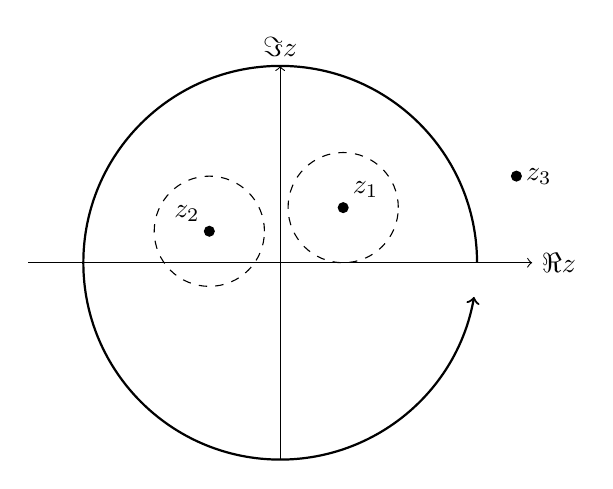
\begin{tikzpicture}[scale=1.0]
    \draw[->] (-3.2,0)--(3.2,0) node[right] {$\Re z$};
    \draw[->] (0,-2.5)--(0,2.5) node[above] {$\Im z$};
    \draw[thick,->] (2.5,0) arc (0:350:2.5);
    \fill (0.8,0.7) circle (2pt) node[above right] {$z_1$};
    \fill (-0.9,0.4) circle (2pt) node[above left] {$z_2$};
    \fill (3.0,1.1) circle (2pt) node[right] {$z_3$};
    \draw[dashed] (0.8,0.7) circle (0.7);
    \draw[dashed] (-0.9,0.4) circle (0.7);
\end{tikzpicture}
\caption{留数围道包含 $z_1$ 与 $z_2$，但不包含 $z_3$。围道积分等于所包围奇点留数之和的 $2\pi i$ 倍，其中还要计入绕数。}
\end{figure}

\begin{remark}
第一幅图刻画保角性：在 $f'(z_0)\neq0$ 的点附近，微小方向被旋转 $\arg f'(z_0)$，并按 $|f'(z_0)|$ 伸缩。第二幅图刻画留数的局部性：整体围道积分由各个被包围奇点任意小邻域内的数据拼合而成。
\end{remark}


\section{结语}

复分析的核心思想可以概括为：复可微性远强于实可微性。Cauchy 积分公式把边界值与内部值联系起来；Taylor 和 Laurent 展开把函数转化为级数；留数定理则把复杂的积分计算化为有限个局部系数的求和。这些工具不仅在纯数学中具有基础地位，也广泛应用于微分方程、物理、信号处理和概率理论。

\textbf{关键词：} 复数，复平面，全纯函数，Cauchy--Riemann 方程，Cauchy 积分公式，Laurent 级数，留数定理。
